\documentclass{article}
\usepackage{tabularx}
\usepackage{amsmath}
\usepackage{graphicx}
\usepackage[margin=2cm]{geometry}
\usepackage{cite}
\usepackage[final]{hyperref}
\usepackage{listings}
\usepackage{here}
\hypersetup{
	colorlinks=true,
	linkcolor=blue,
	citecolor=blue,
	filecolor=magenta,
	urlcolor=blue         
}

\begin{document}

\title{TP02\\Blurred fractal}
\author{Robin Faury}
\date{01/11/2021}
\maketitle

\begin{abstract}
	\begin{figure}[H]
		\centering
		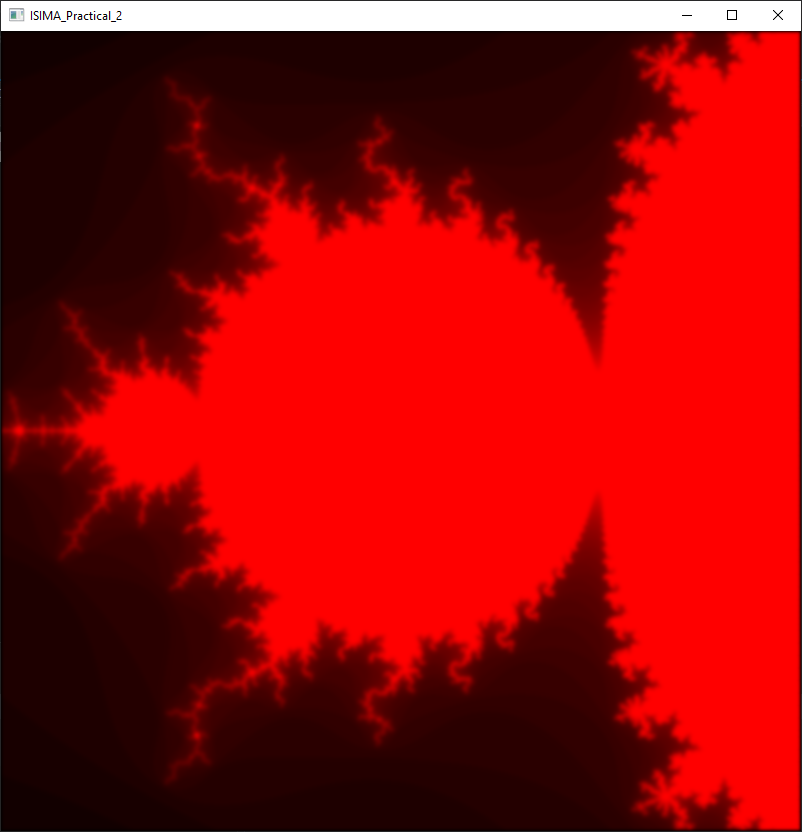
\includegraphics[scale=0.6]{images/Mandelbrot_blur.png}
		\caption{The blurred Mandelbrot set}
	\end{figure}
\end{abstract}

\newpage
\section{Introduction}
\subsection{Cloning the repository}
You can find the source of the practical work by cloning this git repository:
\begin{lstlisting}
	https://github.com/robinfaurypro/GPGPU_ISIMA_2020-2021.git
\end{lstlisting}
The CMakeLists file is stored into the Practical\_2 folder. Open a terminal on this folder and use thus commands:
\begin{lstlisting}
	git submodule update --init
	mkdir build
	cd build
	cmake -G "Visual Studio 15 Win64" ..
\end{lstlisting}
Of course if you are on UNIX system feel free to use the generator you want.
If everything is going well, you can compile and run the executable and get a colored gradient window.

\begin{figure}[h]
	\centering
	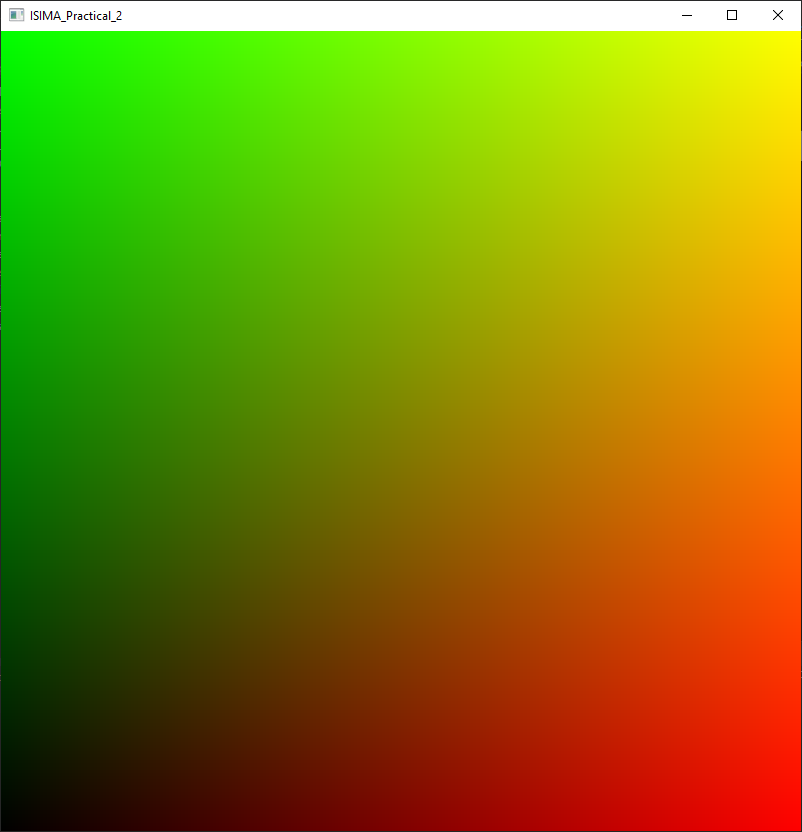
\includegraphics[scale=0.6]{images/uv.png}
	\caption{The UV of a image}
\end{figure}

The UV of a image is simply the coordinate of an image. An image have always UV between 0 and 1. As an example, an image with 1024 pixel on x and 2048 pixels on y get this U and V values: if $U = 0.25$, $X = 128$ and if $V = 0.25$, $Y = 512$.

\section{GPU texture creation}
On the last practical we use a buffer to store some particles and show them on screen. This time our buffer will store each pixel on the image. On the Content struct you can see that the texture\_ item has replace the buffer\_ one. For the moment this handle is set to 0. On the kFragmentSource you can see that we draw the uv coordinate if the texture isn't valid.\\
On the Initialization function we can create the memory space on the GPU memory. First we need to create the handle and bind the texture to work on it:
\begin{lstlisting}
	glGenTextures(1, &content.texture_);
	glBindTexture(GL_TEXTURE_2D, content.texture_);
\end{lstlisting}
Then we need to specify some parameters:
\begin{lstlisting}
	  glTexParameteri(GL_TEXTURE_2D, GL_TEXTURE_WRAP_S, GL_CLAMP_TO_EDGE);
	  glTexParameteri(GL_TEXTURE_2D, GL_TEXTURE_WRAP_T, GL_CLAMP_TO_EDGE);
	  glTexParameteri(GL_TEXTURE_2D, GL_TEXTURE_MAG_FILTER, GL_LINEAR);
	  glTexParameteri(GL_TEXTURE_2D, GL_TEXTURE_MIN_FILTER, GL_LINEAR);
\end{lstlisting}
all parameters can be seen on this well documented tutorial (https://learnopengl.com/Getting-started/Textures).\\
Finally, we can now allocate the memory using this code line and unbind the texture:
\begin{lstlisting}
	  glTexImage2D(
		GL_TEXTURE_2D, 0, GL_RGBA32F, 1024, 1024, 0, GL_RGBA, GL_FLOAT, nullptr);
	glBindTexture(GL_TEXTURE_2D, 0);
\end{lstlisting}
Parameters of the function are:
\begin{itemize}
	\item GL\_TEXTURE\_2D: the target image. You can also manipulate 1D or 3D images.
	\item 0: the level of the texture. In computer graphic, texture can be store along there down scaled version. Here we only use the raw texture.
	\item GL\_RGBA32F: The texture use 32 bits float to store the R, the G, the B and the alpha value. 
	\item 1024: The size on the width.
	\item 1024: The size on the height.
	\item 0: This value must be 0 (https://www.khronos.org/registry/OpenGL-Refpages/gl4/html/glTexImage2D.xhtml).
	\item GL\_RGBA: The format of the pixel. Can also be GL\_BGRA.
	\item GL\_FLOAT: Pixel components are float.
	\item nullptr: a pointer on a CPU data buffer.
\end{itemize}
Because we specify nullptr on the last parameter, the texture will be initialize with null values. If you run you program, you can see the black texture.

\begin{figure}[h]
	\centering
	
\includegraphics[scale=0.2]{images/black.png}
	\caption{A black texture}
\end{figure}

\section{The fractal compute shader}
In the same way you did in the practical 1. Create a new compute shader for the fractal generation named kComputeFractalSource.
The binding of the texture can be done like this:
\begin{lstlisting}
	  layout(rgba32f, binding=0) uniform image2D texture_fractal;
\end{lstlisting}
We can use the feature of a 2D layout for the organization of our threads:
\begin{lstlisting}
	 layout(local_size_x = 8, local_size_y = 8, local_size_z = 1) in;
\end{lstlisting}
The value 8 was chosen to keep all shader invocations of a bloc inside a warp (8x8=32 threads). Finally, read and write on the texture can be done using imageLoad and imageStore. We can use the main function to show all the local invocation shader:
\begin{lstlisting}
void main() {
	ivec2 coord = ivec2(gl_GlobalInvocationID.xy);
	imageStore(
		texture_fractal,
		coord,
		vec4(vec2(gl_LocalInvocationID.xy)/32.0, 0.0, 1.0));
}
\end{lstlisting}
On the CPU side we can use the program and the texture like on the first practical. The dispatch function will set 128 on Y too:
\begin{lstlisting}
glUseProgram(content.kernel_compute_blur_);
glBindTexture(GL_TEXTURE_2D, content.texture_);
glBindImageTexture(
  0, content.texture_, 0, GL_FALSE, 0, GL_WRITE_ONLY, GL_RGBA32F);
glDispatchCompute(128, 128, 1);
glMemoryBarrier(GL_SHADER_IMAGE_ACCESS_BARRIER_BIT);
glBindImageTexture (0, 0, 0, GL_FALSE, 0, GL_WRITE_ONLY, GL_RGBA32F);
glBindTexture(GL_TEXTURE_2D, 0);
glUseProgram(0);
\end{lstlisting}

\begin{figure}[h]
	\centering
	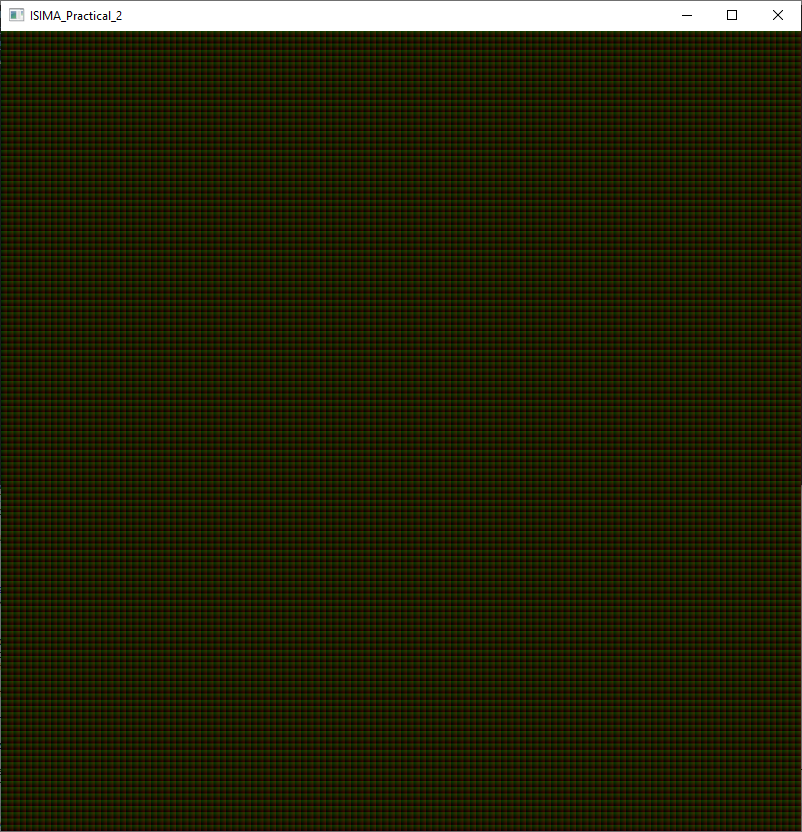
\includegraphics[scale=0.4]{images/local_uv.png}
	\caption{Print local UV on a image using a compute shader}
\end{figure}

\section{The Mandelbrot set}
The Mandelbrot set is the set of complex numbers $c$ for which the function
\begin{equation}
f_c(z) = z^2+c
\end{equation}
does not diverge when iterated from $z = 0+0i$.\\
As a reminder complex number multiplication is:
\begin{equation}
z_1*z_2 = (z_1.real*z_2.real-z_1.imag*z_2.imag) + (z_1.real*z_2.imag + z_1.imag*z_2.real)*i
\end{equation}
The addition is:
\begin{equation}
z_1 + z_2 = (z_1.real + z_2.real) + (z_1.imag + z_2.imag)*i
\end{equation}
And the modulus of a complex is his length or magnitude.\\
We can run the equation $(1)$ while the result don't diverge. We consider a complex number is outside of the [-2; 2] window is a divergent value. $iterationMax$ is the number max of "jump".
\begin{lstlisting}
	float iteration_max = 42.0;
	float iteration = 0.0;
	while (z.modulus() < 2 && iteration <= iteration_max) {
		z = z*z + c;
		++iteration;
	}
\end{lstlisting}
If iteration reach iteration\_max that means the complex number chosen is part of the Mandelbrot set. We can use the iteration value as a color to show the fractal.
\begin{lstlisting}
	vec4 color = vec4(iteration/iteration_max, 0.0, 0.0, 1.0)
\end{lstlisting}
For the generation of the Mandelbrot set we will use $c = -1.5 - 0.5i$.
\begin{lstlisting}
	vec2 c = vec2(float(coord.x)/1024.0-1.5, float(coord.y)/1024.0-0.5);
\end{lstlisting}
Implement this algorithm to generate a fractal into the texture and show it:

\begin{figure}[h]
	\centering
	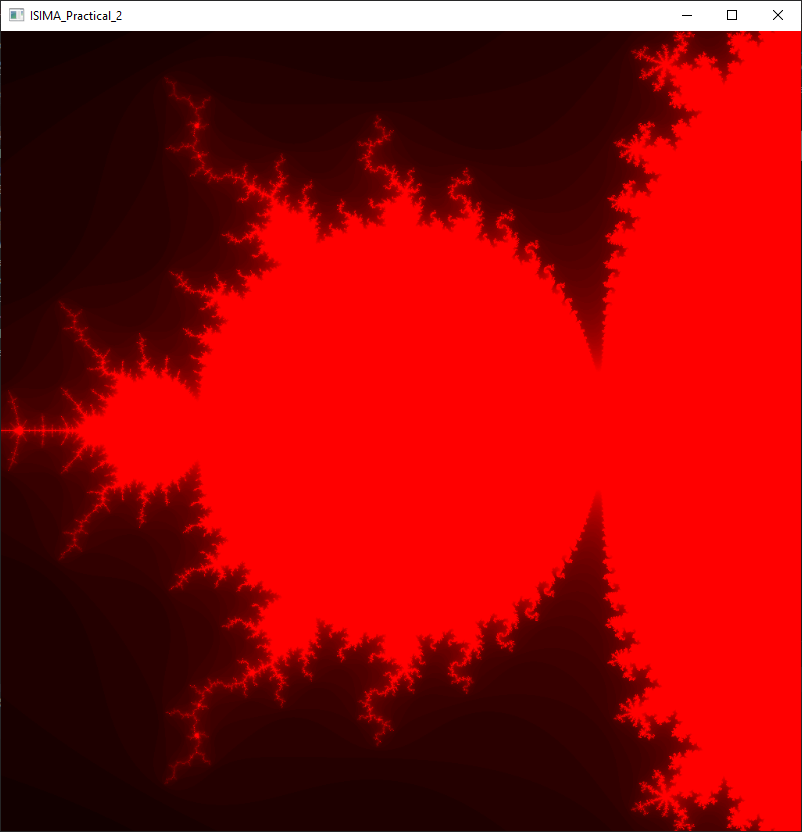
\includegraphics[scale=0.4]{images/Mandelbrot.png}
	\caption{Mandelbrot set}
\end{figure}

\section{The blur compute shader}
On the last shader we write values into the texture. On this section we will read and write pixels. This operation can be done easily but the blur algorithm need neighborhood pixels. So sometime you will read pixel and sometime you will read modified pixel. To prevent that we can use the barrier key word.\\
Create another compute shader named kComputeBlurSource that compute the mean of the 9 neighborhood pixels by reading the input texture (imageLoad). Use the barrier(); function before write in the texture (imageStore).
By applying this process 10 time you can get this result:
\begin{figure}[H]
	\centering
	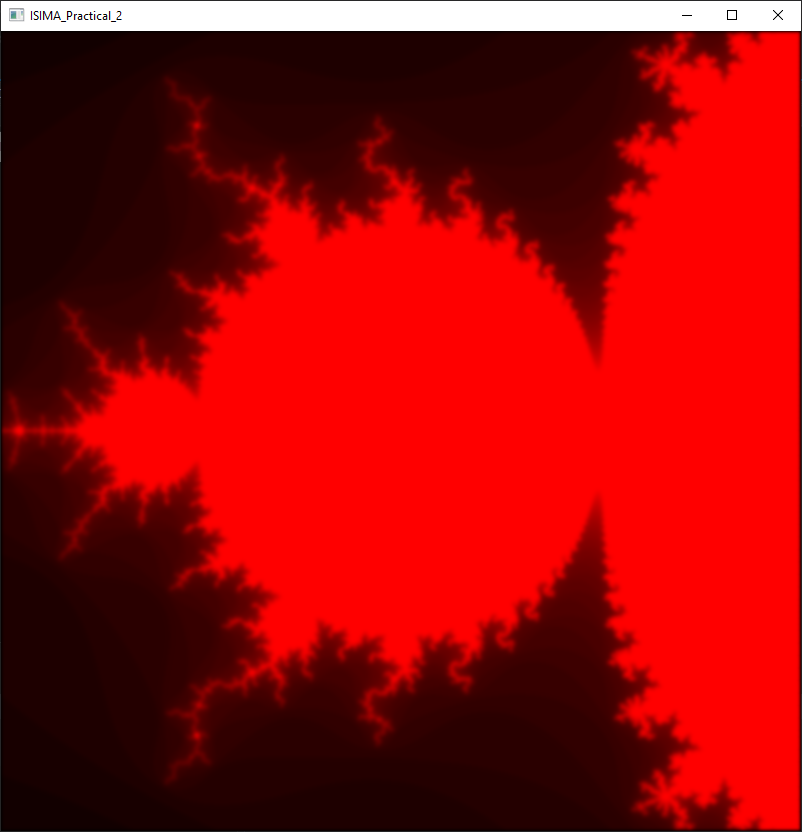
\includegraphics[scale=0.6]{images/Mandelbrot_blur.png}
	\caption{The blurred Mandelbrot set}
\end{figure}

\section{Bonus}
Implement the Julia Set using the same algorithm but with this parameter at start:
\begin{itemize}
	\item z = x/width + (y/height)*i
	\item c = 0.292 + 0.015*i
	\item iteration\_max = 400
\end{itemize}

\end{document}